\documentclass[11pt]{article}

\usepackage[a4paper,margin=2.5cm]{geometry}
\usepackage{amsmath}
\usepackage{graphicx}
\usepackage{booktabs}
\usepackage{array}
\usepackage{xcolor}
\usepackage{tikz}
\usepackage{hyperref}
\usepackage{enumitem}
\usepackage{fancyhdr}
\usetikzlibrary{arrows.meta, positioning}

\hypersetup{colorlinks=true, linkcolor=blue, urlcolor=blue, citecolor=blue}

\pagestyle{fancy}
\setlength{\headheight}{14pt}
\fancyhf{}
\fancyhead[L]{EVKA Position -- Laser Radius Study}
\fancyhead[R]{\thepage}
\renewcommand{\headrulewidth}{0.4pt}

% ---- placeholder box for a hardware photo the user will add later ----
% Usage: \photoplaceholder{Device Name}{images/filename.jpg}
% To swap in a real photo later: replace the \photoplaceholder{...}{...} call
% with \includegraphics[width=0.6\linewidth]{images/filename.jpg} once the
% file exists under report/images/.
\newcommand{\photoplaceholder}[2]{%
  \begin{center}
  \begin{tikzpicture}
    \draw[thick, dashed, gray] (0,0) rectangle (6,3.6);
    \node[align=center, text width=5.5cm, gray] at (3,2.0) {\footnotesize Photo placeholder};
    \node[align=center, text width=5.5cm] at (3,1.1) {\small #1};
    \node[align=center, text width=5.5cm, gray, font=\tiny] at (3,0.4) {drop image at \texttt{#2}};
  \end{tikzpicture}
  \end{center}
}

\title{\textbf{Laser Radius Sensor Selection}\\[0.3em]
\large EVKA Spherical Positioning System --- Requirement Study}
\author{EVKA Position Project}
\date{2026-07-01}

\begin{document}
\maketitle

% ===================================================================
\section{Requirement and Scope}
% ===================================================================

The EVKA system computes 3D position from spherical coordinates $(r,\theta,\phi)$, converted to Cartesian $(X,Y,Z)$ via the elevation-azimuth convention already used in production firmware. Two rotary encoders (Autonics E40S6-5000, 20{,}000 pulses/rev via X4 quadrature) measure $\theta$ and $\phi$ and are unchanged by this study. Only the radius source changes: from draw-wire quadrature counts to a laser distance reading.

\textbf{Fixed requirement (confirmed with the project owner):}
\begin{itemize}[nosep]
  \item Maximum range: \textbf{40\,m}
  \item Laser device accuracy: \textbf{$\leq$10\,mm}, target sub-centimeter, across the full 0--40\,m range
  \item This is the \emph{laser device's own datasheet accuracy}, a hardware-selection filter --- not the total combined-system XYZ accuracy (see Section~\ref{sec:budget})
\end{itemize}

Two mounting variants remain in scope, unchanged from the project's original design decisions:

\begin{description}[leftmargin=1.2cm]
  \item[Version A] Detachable handheld laser, docked on the phi head, quick-disconnect for standalone field use. Wired serial preferred; Bluetooth LE (BLE) is an acceptable fallback.
  \item[Version B] Permanently mounted fixed module on the phi head, no operator handling, automation-first.
\end{description}

% ===================================================================
\section{Methodology: Why Accuracy Class, Not Just Price, Filters the Shortlist}
% ===================================================================

\label{sec:methodology}
Laser distance measurement in this price/size class comes in two fundamentally different techniques:

\begin{description}[leftmargin=1.4cm]
  \item[Pulsed time-of-flight (ToF)] Measures the direct round-trip travel time of a light pulse. A 40\,m round trip takes $\approx$267\,ns; achieving millimeter-class accuracy over that interval requires sub-nanosecond timing resolution, which low-cost ToF modules (Benewake TF-series, DFRobot SEN0492, and similar) do not have. These modules report accuracy in the \textbf{centimeter-to-decimeter} range: $\pm$5\,cm at short range, $\pm$1\% of reading at long range (i.e.\ $\pm$400\,mm at 40\,m).
  \item[Phase-shift / AMCW (Amplitude-Modulated Continuous Wave)] Modulates the beam and measures the phase difference of the reflected signal. This yields \textbf{flat, distance-independent} accuracy across a device's full rated range --- typically $\pm$1--2\,mm regardless of whether the target is at 1\,m or 40\,m. This is how essentially every construction-grade handheld laser distance meter (Leica; and, industry-typically, Bosch) and industrial OEM ``laser distance sensor'' module (Meskernel, Dimetix) works --- though the Bosch and JRT lines are \emph{flagged} in Section~\ref{sec:devices} because a primary-source confirmation of their principle is still missing.
\end{description}

Figure~\ref{fig:accuracy_vs_range} and the device table in Section~\ref{sec:devices} make this concrete: every phase-shift candidate stays flat and well under the 10\,mm line across the full range, while the pulsed-ToF class (previously the primary recommendation under an earlier, tiered version of this study) is 5--40$\times$ over budget for most of the range.

\begin{figure}[htbp]
  \centering
  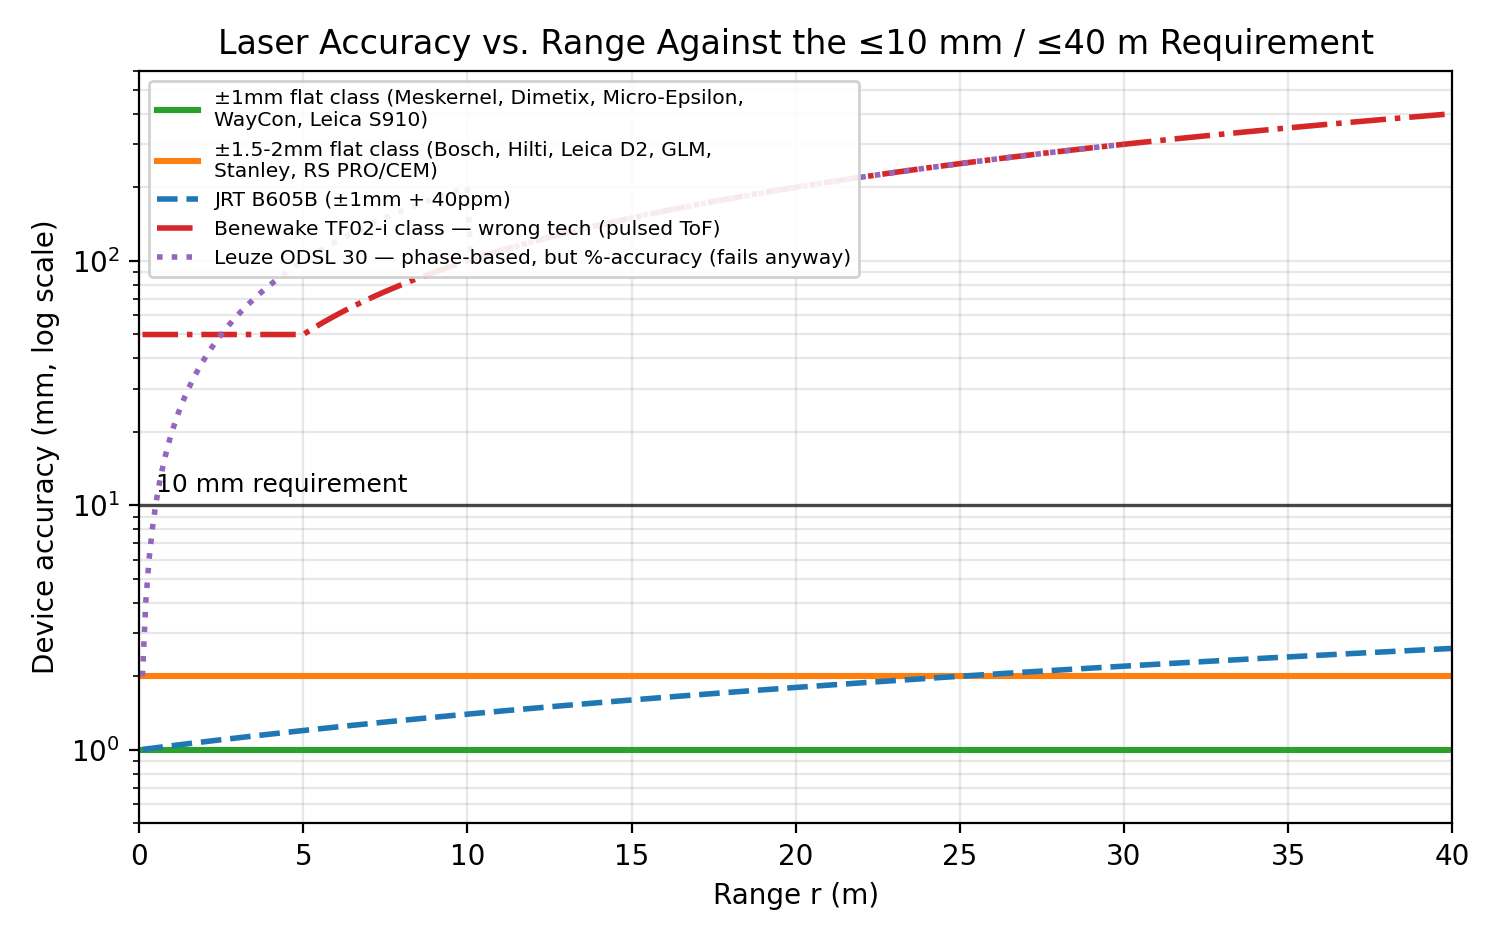
\includegraphics[width=0.85\linewidth]{figures/accuracy_vs_range.png}
  \caption{Device accuracy vs. range (log scale) against the 10\,mm requirement. Phase-shift devices stay flat and well under budget; the pulsed-ToF class (Benewake TF02-i and similar) fails the spec almost everywhere except very short range.}
  \label{fig:accuracy_vs_range}
\end{figure}

% ===================================================================
\section{Kinematic Chain}
% ===================================================================

The laser replaces the draw-wire in the existing kinematic chain without altering the role of the two rotary encoders:

\begin{center}
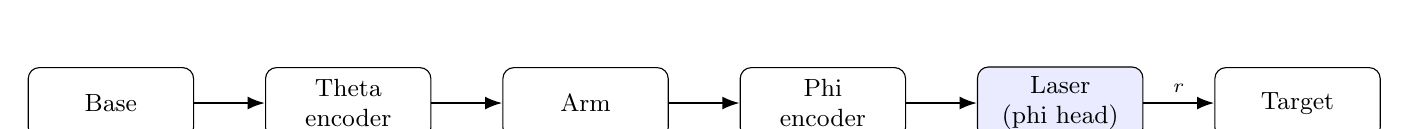
\begin{tikzpicture}[
    node distance=1.15cm and 0.9cm,
    box/.style={draw, rounded corners, minimum width=2.1cm, minimum height=0.9cm, align=center, font=\small},
    arr/.style={-{Latex[length=2.2mm]}, thick}
  ]
  \node[box] (base) {Base};
  \node[box, right=of base] (theta) {Theta\\encoder};
  \node[box, right=of theta] (arm) {Arm};
  \node[box, right=of arm] (phi) {Phi\\encoder};
  \node[box, right=of phi, fill=blue!8] (laser) {Laser\\(phi head)};
  \node[box, right=of laser] (target) {Target};

  \draw[arr] (base) -- (theta);
  \draw[arr] (theta) -- (arm);
  \draw[arr] (arm) -- (phi);
  \draw[arr] (phi) -- (laser);
  \draw[arr] (laser) -- node[above, font=\scriptsize] {$r$} (target);
\end{tikzpicture}
\end{center}

The laser's optical reference plane sits a fixed offset $d_{\text{offset}}$ forward of the phi rotation axis (mounting bracket standoff); the true radius is $r_{\text{true}} = r_{\text{laser}} + d_{\text{offset}}$, a one-time additive calibration constant --- simpler than the draw-wire's multiplicative PPR/drum-circumference scale, since phase-shift devices already report calibrated millimeters. Full geometry and a proposed \texttt{CAL\_R}/\texttt{ZERO\_R} calibration workflow (replacing the current \texttt{CAL\_W}) are in \texttt{kinematics\_and\_calibration.md}.

% ===================================================================
\section{Device Shortlist}
\label{sec:devices}
% ===================================================================

\subsection{Original Shortlist}

\begin{table}[htbp]
\centering
\small
\begin{tabular}{@{}p{2.4cm}p{1.5cm}p{2.0cm}p{2.9cm}p{2.0cm}p{2.0cm}@{}}
\toprule
\textbf{Device} & \textbf{Range} & \textbf{Accuracy} & \textbf{Interface} & \textbf{Role} & \textbf{Price} \\
\midrule
Meskernel LDL-T & 0.03--80\,m & $\pm$1\,mm flat, 100\,Hz & USART / RS232 / RS485 & A or B (bare module) & \$87.50 conf. \\
Dimetix DBN-50-050 & 0.05--50\,m & $\pm$5\,mm flat & RS232 / RS422, \textbf{public ASCII} & B (industrial) & \$1{,}332 conf. \\
Dimetix DAE-10-050 & 0.05--50\,m & $\pm$1\,mm flat & RS232 / RS422, \textbf{public ASCII} & B (industrial) & \$2{,}700 conf. \\
Leica DISTO D5 & 0.05--200\,m & $\pm$1\,mm flat & BLE 5.0 + USB-C & A (handheld) & \$311--708 conf. \\
JRT B605B / M88B$^\dagger$ & 0.03--150\,m & $\approx\pm$2.6\,mm @ 40\,m & RS232 TTL & A or B (flagged) & \$43--90 est. \\
Bosch PLR 40\,C$^\dagger$ & 0.05--40\,m & $\pm$2\,mm flat & BLE 4.2 only & A (flagged) & \$110--125 conf. \\
\bottomrule
\end{tabular}
\caption{Devices meeting the $\leq$10\,mm / $\leq$40\,m requirement, original shortlist (prices from the 2026-07-08 Istanbul survey). $^\dagger$ = phase-shift principle \emph{not independently confirmed}; held out of the certified pass list until a primary-source datasheet verifies it (not excluded --- it is not ToF/\%-of-reading).}
\end{table}

\subsection{Extended Shortlist --- 2026-07-01 Addendum}

A follow-up research pass, assisted by a GitHub Copilot CLI research agent, swept 20+ additional manufacturers (handheld tool brands and industrial automation sensor vendors) specifically filtering for phase-shift/AMCW technology. This found 12 more qualifying devices; the 2026-07-08 Istanbul price survey then added three more (Leica DISTO~X6, Dimetix DBN-50-050, FAE LS~121/122~FA), bringing the qualifying/flagged total to 20. The standouts are listed below; the complete list, plus a documented ``don't re-research these'' list of 15+ rejected devices and manufacturers, is in \texttt{version\_a\_handheld\_devices.md}~\S3 and \texttt{version\_b\_integrated\_modules.md}~\S3.

\begin{table}[htbp]
\centering
\small
\begin{tabular}{@{}p{2.4cm}p{1.7cm}p{1.4cm}p{2.8cm}p{2.0cm}p{2.0cm}@{}}
\toprule
\textbf{Device} & \textbf{Range} & \textbf{Accuracy} & \textbf{Interface} & \textbf{Role} & \textbf{Price} \\
\midrule
Leica DISTO S910 & 0.05--300\,m & $\pm$1.0\,mm & BLE + WLAN + \textbf{native USB} & A --- best spec & \$1{,}916--2{,}132 conf. \\
Leica DISTO X6 \textbf{[NEW]} & 0.05--250\,m & $\pm$1.0\,mm & BLE + USB-C & A --- rugged flagship & \$2{,}263 conf. \\
RS PRO ILDM-150H & 0.05--70\,m & $\pm$1.5\,mm & BLE 4.0 & A --- cheapest BLE & \$90--130 est. \\
Hilti PD-I & 0.05--100\,m & $\pm$1.5\,mm & Bluetooth & A (premium) & \$400--500 est. \\
Micro-Epsilon ILR2250/3800 & up to 150\,m & $\pm$1\,mm lin. & RS422 / USB, fieldbus adapters & B (industrial) & \$1{,}800 est. \\
FAE LS 121/122 FA \textbf{[NEW]} & 50\,m & $\pm$3\,mm & RS232 / RS422 (ASCII) & B (industrial) & \$1{,}400 est. \\
Jenoptik LDM41 & 150\,m refl.\ / $\sim$30\,m nat. & $\leq$3\,mm flat & RS232 / 422 / Profibus / SSI & B (industrial) & \$1{,}500 est. \\
WayCon LDI & 0.05--100\,m (500\,m refl.) & $\pm$1\,mm, $\pm$0.3\,mm rep. & 4--20\,mA, RS232 / 422 / 485 / SSI & B (industrial) & Quote-only \\
\bottomrule
\end{tabular}
\caption{Standout devices from the extended pass, with 2026-07-08 confirmed/estimated prices. Micro-Epsilon, FAE and WayCon are industrial alternatives to Dimetix; Jenoptik's 150\,m headline is reflector-dependent ($\sim$30\,m on natural surfaces). Micro-Epsilon's older ILR1171/1191 line was corrected to pulsed ToF and rejected.}
\end{table}

\textbf{Caution:} not every phase-based industrial sensor meets the flat-mm bar --- the Leuze ODSL~30 uses genuine phase-based ranging but its published accuracy is percentage-of-reading (1--2\% FS), which works out to $\approx\pm$100--300\,mm at 10--30\,m. It is documented in \texttt{version\_b\_integrated\_modules.md}~\S3.1 as a flagged near-miss, not a recommendation --- see Figure~\ref{fig:accuracy_vs_range}.

\subsection{Cost and Sourcing (2026-07-08 survey)}
\label{sec:sourcing}

The 2026-07-08 price survey turns the earlier estimate-heavy shortlist into mostly confirmed pricing, which makes the real decision visible: at a fixed $\pm$1\,mm accuracy, delivered price spans from $\approx$\$43 (Meskernel/JRT OEM modules) to $\approx$\$2,772 (Dimetix DAE-10-050, Leica X6/S910) --- roughly a 60$\times$ spread for the \emph{same accuracy figure} (Figure~\ref{fig:price_vs_accuracy}). Accuracy is never what you pay for; housing, brand, and certification are. The second axis of the decision is sourcing: only the Leica handhelds and the (flagged) Bosch units are in-stock domestically in Turkey; the confirmed-phase-shift OEM and industrial leads (Meskernel, Dimetix) are import/EU-order with multi-week lead times (Figure~\ref{fig:turkey_availability}).

\begin{figure}[htbp]
  \centering
  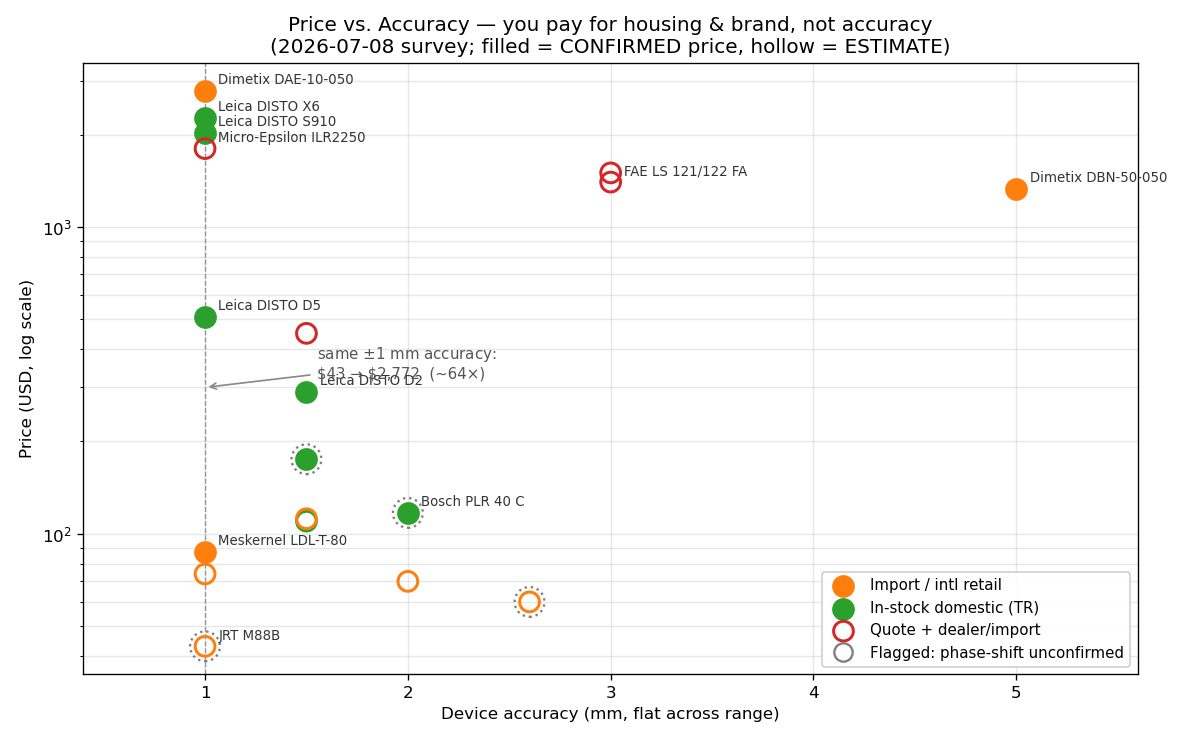
\includegraphics[width=0.85\linewidth]{figures/price_vs_accuracy.png}
  \caption{Price vs.\ device accuracy (log price). Filled markers are CONFIRMED prices, hollow are ESTIMATE; colour is Turkey sourcing class. The dotted ring marks the two devices (Bosch, JRT) whose phase-shift principle is unconfirmed. At $\pm$1\,mm the price spans \$43--\$2,772.}
  \label{fig:price_vs_accuracy}
\end{figure}

\begin{figure}[htbp]
  \centering
  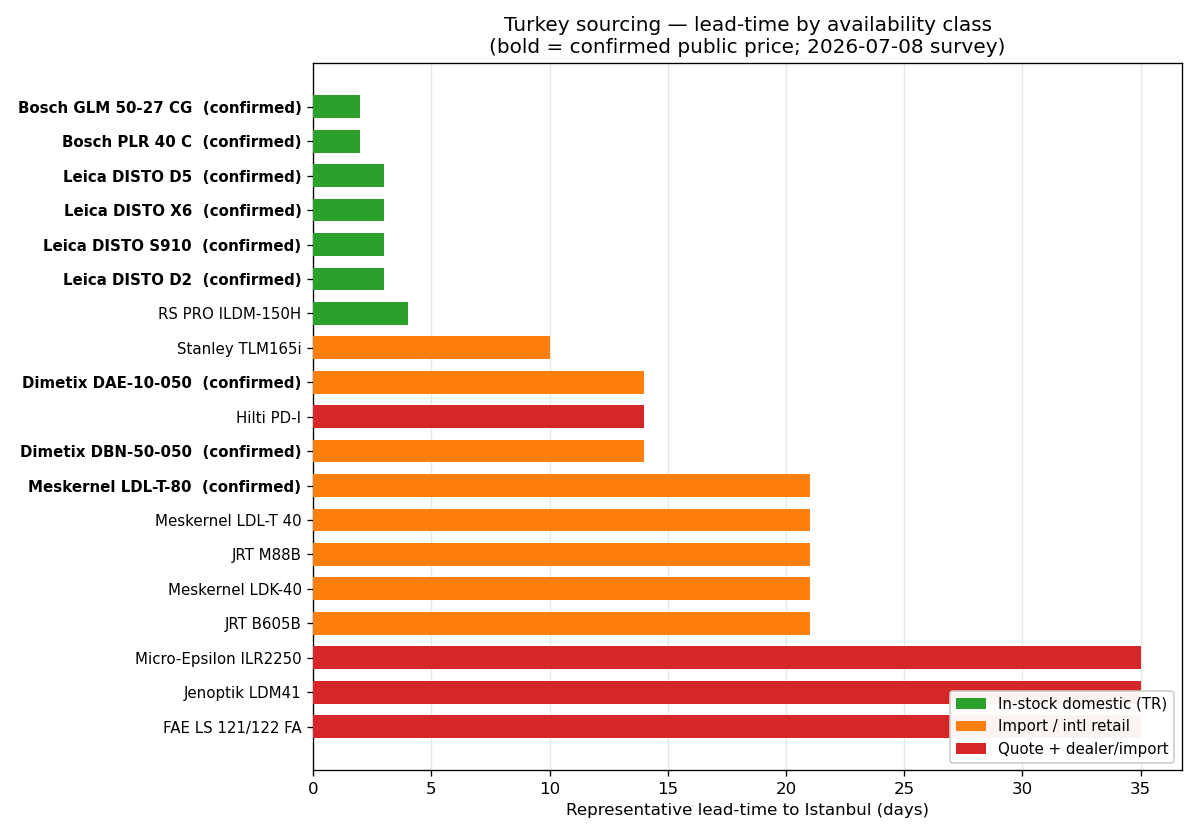
\includegraphics[width=0.85\linewidth]{figures/turkey_availability.png}
  \caption{Representative lead-time to Istanbul by sourcing class. Bold labels have a confirmed public price. The confirmed-phase-shift leads (Meskernel, Dimetix) are import/EU-order; only Leica (and the flagged Bosch) are domestically stocked.}
  \label{fig:turkey_availability}
\end{figure}

\begin{figure}[htbp]
  \centering
  \begin{minipage}[b]{0.40\linewidth}
    \centering
    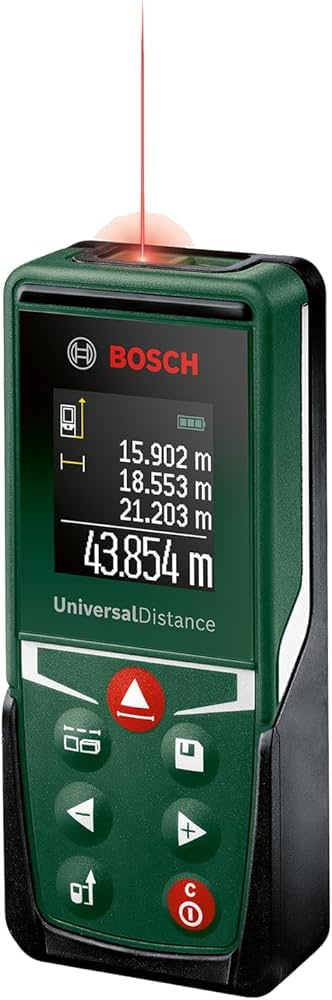
\includegraphics[height=5.5cm]{images/bosch_plr40c.jpg}
  \end{minipage}
  \hfill
  \begin{minipage}[b]{0.40\linewidth}
    \centering
    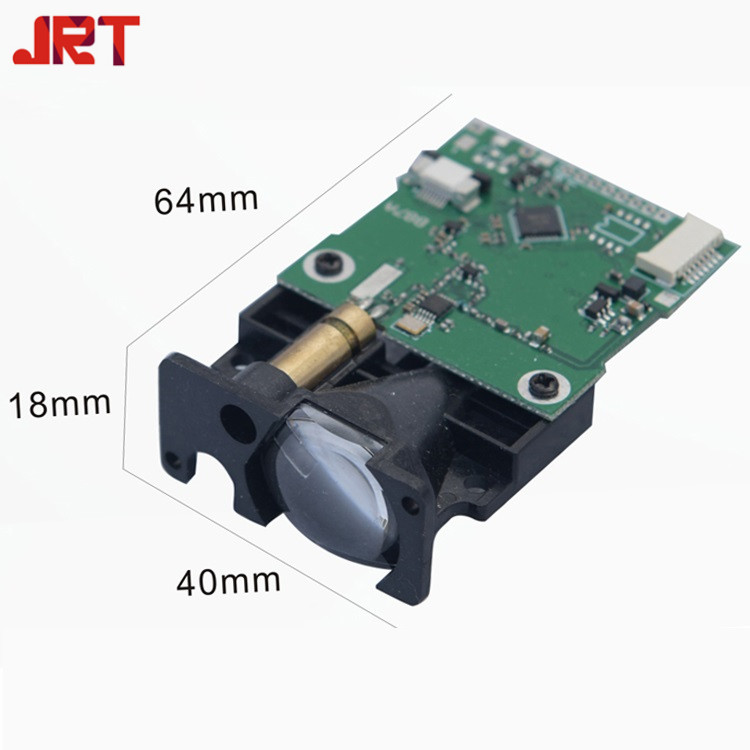
\includegraphics[height=5.5cm]{images/jrt_b605b.jpg}
  \end{minipage}
  \caption{The two \textbf{flagged} devices, kept as references pending a primary-source phase-shift confirmation. Left: Bosch PLR 40\,C (fast domestic BLE, principle unconfirmed). Right: JRT B605B bare module (cheapest wired, principle unconfirmed).}
\end{figure}

\subsection{Devices Excluded (Fail the Spec)}

The previous version of this study (before the requirement was fixed to a single $\leq$10\,mm/$\leq$40\,m spec) recommended the Benewake TF02-i-RS485 as its primary Version~B pick. Under the current requirement it --- and every pulsed-ToF alternative considered (TF03, TFmini-S/Plus, DFRobot SEN0492) --- is excluded:

\begin{table}[htbp]
\centering
\small
\begin{tabular}{@{}lll@{}}
\toprule
\textbf{Device} & \textbf{Accuracy} & \textbf{Why it fails} \\
\midrule
Benewake TF02-i-RS485 & $\pm$5\,cm ($<$5\,m), $\pm$1\% (5--25\,m) & Pulsed ToF; 5--40$\times$ over the 10\,mm budget \\
Benewake TF03 & $\pm$10\,cm ($<$10\,m), $\pm$1\% ($>$10\,m) & Pulsed ToF; same limitation, longer range only \\
DFRobot SEN0492 & $\pm$2\,cm & Pulsed ToF; also only 4\,m max range \\
\bottomrule
\end{tabular}
\caption{Excluded pulsed-ToF devices and the physics reason (Section~\ref{sec:methodology}), not a bare exclusion.}
\end{table}

% ===================================================================
\section{Combined System Error Budget (Context, Out of Scope)}
% ===================================================================
\label{sec:budget}

The $\leq$10\,mm requirement applies to the laser device's own spec, not the total combined XYZ position accuracy --- confirmed as out of scope for this study. It is still worth surfacing: the rotary encoders' angular resolution contributes an arc-length error that \emph{grows linearly with range} ($\approx r \times 3.14\times10^{-4}$ at 0.018\textdegree/pulse), reaching $\approx$12.6\,mm per axis at 40\,m ($\approx$17.8\,mm combined RSS across both axes). Figure~\ref{fig:error_budget} shows that past roughly 15\,m, the \emph{choice of laser stops mattering much} to total system accuracy --- the encoders dominate regardless of which $\leq$10\,mm-class device is picked. If total system accuracy at long range is ever required (not just laser-device accuracy), the bottleneck shifts to encoder resolution, not laser selection.

\begin{figure}[htbp]
  \centering
  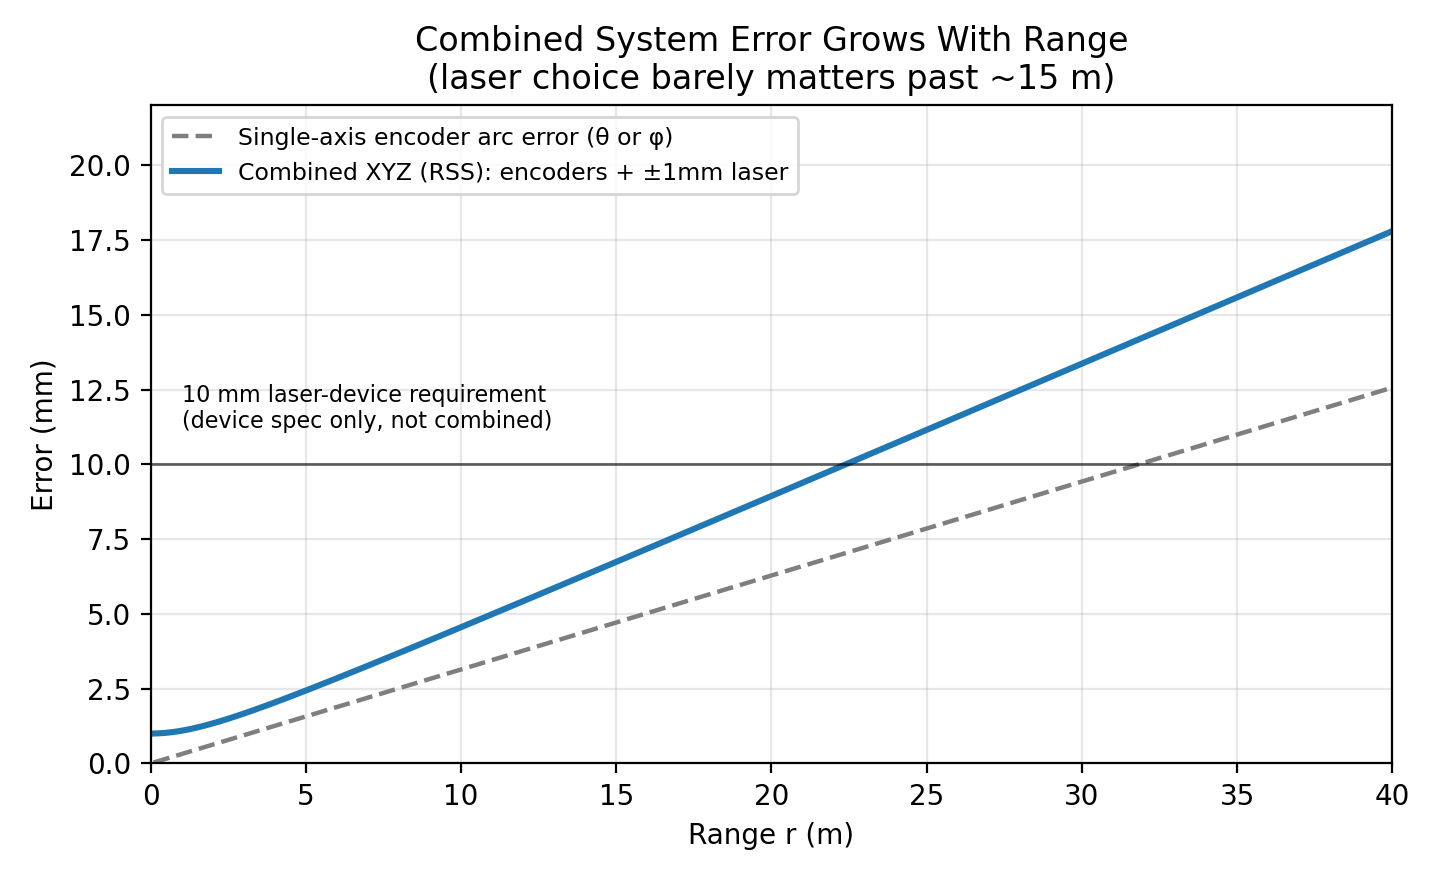
\includegraphics[width=0.82\linewidth]{figures/error_budget.png}
  \caption{Combined system error (RSS of both encoder axes plus a representative $\pm$1\,mm laser) vs.\ range. The encoder contribution alone approaches the 10\,mm line by $\sim$15\,m and exceeds it well before 40\,m, independent of laser accuracy.}
  \label{fig:error_budget}
\end{figure}

% ===================================================================
\section{Recommendation and Bench-Test Order}
% ===================================================================

Revised 2026-07-08 to lead with \emph{confirmed-phase-shift} devices; the earlier draft led with Bosch and JRT, now flagged because the stricter survey could not confirm their measurement principle.

\begin{enumerate}[nosep]
  \item \textbf{Meskernel LDL-T} --- order first. The cheapest device with \emph{both} a confirmed phase-shift principle and a confirmed street price (\$87.50 for the 80\,m LDL-T-80); $\pm$1\,mm, 100\,Hz native (exceeds the 20\,Hz loop). Request its command datasheet before ordering --- the byte-level protocol is the one open gap. The bare module works docked (Version~A) or panel-mounted (Version~B).
  \item \textbf{Dimetix DBN-50-050} (\$1{,}332, $\pm$5\,mm) --- order alongside. It is the only candidate with a fully \textbf{public ASCII protocol}, so it de-risks the firmware parsing path independently; step up to \textbf{DAE-10-050} (\$2{,}700, $\pm$1\,mm) only if the tighter accuracy is wanted.
  \item \textbf{Leica DISTO D5} (\$311--708, confirmed in TR) --- a confirmed-phase-shift $\pm$1\,mm handheld reference and a clean way to validate the BLE read path (unlike the flagged Bosch).
  \item \textbf{Flagged --- Bosch PLR 40\,C, RS PRO ILDM-150H, JRT B605B/M88B} --- cheap and fast/domestic, but order only \emph{after} a primary-source datasheet confirms the phase-shift principle. Until then, keep the Bosch as a hand reference only.
  \item \textbf{Industrial tier --- Micro-Epsilon ILR2250 (\$1{,}800), WayCon LDI, or FAE LS 121/122 FA (\$1{,}400)} --- conditional, only if IP-rated/certified housing becomes a hard requirement; request quotes in parallel rather than defaulting to one vendor.
\end{enumerate}

Full pricing table, supplier list, and reasoning: \texttt{procurement\_and\_bom.md}.

% ===================================================================
\section{Open Risks}
% ===================================================================

\begin{itemize}[nosep]
  \item \textbf{Bosch and JRT phase-shift principle unconfirmed} --- both flagged (Section~\ref{sec:devices}); confirm from a primary-source datasheet before certifying either.
  \item Meskernel's byte-level protocol is not cleanly public (its price is now confirmed) --- a datasheet request is required before firmware implementation.
  \item Dimetix SKU is now resolved (DAE-10-050 / DBN-50-050, confirmed prices); only a Turkey shipping quote and the ESTIMATE-only industrial prices (Micro-Epsilon \$1{,}800, Jenoptik \$1{,}500, FAE \$1{,}400, WayCon quote-only) remain to confirm. Confirmed TL prices are FX/VAT-sensitive (USD/TRY 46.85, 2026-07-08).
  \item The RS-485/RS422 wiring plan repurposes GPIO pins (13/14/15) that differ from the older \texttt{12v\_legacy/v2} pin map originally cited for this variant; the current as-built 5V v2 carrier board wires those pins differently and has no onboard RS-485/RS422 transceiver yet --- an open item for PCB-owner review, not yet implemented.
  \item The combined-system accuracy at 40\,m ($\approx$18\,mm, Section~\ref{sec:budget}) is out of scope per the current decision but should be revisited if total XYZ accuracy at long range ever becomes a requirement.
\end{itemize}

% ===================================================================
\section{Conclusion}
% ===================================================================

The $\leq$40\,m / $\leq$10\,mm requirement is comfortably achievable, but only with phase-shift laser distance measurement --- the pulsed-ToF modules that looked attractive under a looser, tiered accuracy target no longer qualify. A follow-up research sweep across 20+ manufacturers, plus the 2026-07-08 price survey, grew the qualifying/flagged shortlist from 5 to 20 devices without changing that core conclusion: the requirement is easy to meet, and the interesting decisions are about price, mounting, sourcing, and interface, not accuracy (Figures~\ref{fig:price_vs_accuracy}--\ref{fig:turkey_availability}). A cheap bench-test path led by a \emph{confirmed}-phase-shift device --- Meskernel LDL-T, plus the public-protocol Dimetix DBN-50-050 and a Leica DISTO D5 handheld reference --- can validate the integration approach for a fraction of the cost of any industrial-grade alternative (Micro-Epsilon, WayCon, FAE), which should be reserved for cases where certified housing, not accuracy, is the deciding factor. The popular Bosch and JRT modules remain attractive on price but are held out of the certified list until their measurement principle is confirmed. Full technical detail, per-device protocol notes, the proposed calibration workflow, and the firmware integration sketch are maintained in the linked markdown files under \texttt{laser\_radius/} in the project repository, which remains the authoritative source --- this report is a condensed summary of that work.

\vspace{1em}
\noindent\textit{Docs-only study --- no firmware or PCB files were changed. Additional hardware photographs can be added under \texttt{report/images/} following the pattern already used for the Bosch and JRT photos above (see the comment at the top of \texttt{report.tex} for the \texttt{\textbackslash includegraphics} snippet).}

\end{document}
